\section{Results}

\subsection{Primary external performance}
The primary evaluation included \ProbeRuns{} selected checkpoints and
\ExternalPredictions{} predictions for \PrimarySubjects{} MIPDB participants.
The baseline achieved mean Pearson correlation \BaselinePearson{}, MAE
\BaselineMAE{} years, and RMSE \BaselineRMSE{} years
(Table~\ref{tab:absolute-metrics}). The rich-statistics head had the highest
mean correlation, while the multi-query head had the lowest MAE and RMSE.
All four heads had negative $R^2$ and calibration slopes above one, indicating
substantial absolute error despite positive correlations.

\begin{table}[tbp]
  \centering
  \small
  \caption{Mean MIPDB metrics across ten training seeds. MAE and RMSE are in
  years. Calibration fits observed age against predicted age.}
  \label{tab:absolute-metrics}
  % Generated table; do not edit.
\begin{tabular}{lrrrrr}
\toprule
Head & Pearson & MAE & RMSE & R-squared & Cal. slope \\
\midrule
Mean-pooled linear & 0.644 & 3.241 & 3.961 & -0.674 & 1.706 \\
Penultimate-layer linear & 0.653 & 3.297 & 4.008 & -0.714 & 1.750 \\
Rich-statistics residual & 0.676 & 2.563 & 3.323 & -0.180 & 1.802 \\
Multi-query rich-statistics & 0.654 & 2.373 & 3.144 & -0.057 & 1.489 \\
\bottomrule
\end{tabular}

\end{table}

\subsection{Paired primary comparisons}
Mean Pearson differences from the matched baseline were
\LayerLinearPearsonDelta{} for the penultimate-layer linear probe,
\RichResidualPearsonDelta{} for the rich-statistics head, and
\MultiQueryPearsonDelta{} for the multi-query head. All three Holm-adjusted
sign-flip p-values were below 0.05. However, every joint bootstrap interval
included zero (Table~\ref{tab:confirmatory} and Figure~\ref{fig:bootstrap}), so
none met all conditions of the prespecified decision rule.

\begin{table}[tbp]
  \centering
  \small
  \caption{Primary paired differences from the final-layer linear baseline.
  Intervals resample seeds and participants. W/T/L counts positive, zero, and
  negative seed differences; Stable denotes passing all five decision criteria.}
  \label{tab:confirmatory}
  % Generated table; do not edit.
\begin{tabular}{lrrrrrr}
\toprule
Candidate & Mean diff & 95\% CI & Holm-adjusted p & W/T/L & Worst & Stable \\
\midrule
Penultimate layer & 0.008 & [-0.019,\ 0.036] & 0.003 & 10/0/0 & 0.004 & no \\
Rich residual & 0.032 & [-0.050,\ 0.125] & 0.003 & 10/0/0 & 0.025 & no \\
Multi-query & 0.010 & [-0.114,\ 0.154] & 0.004 & 8/0/2 & -0.003 & no \\
\bottomrule
\end{tabular}

\end{table}

\begin{figure}[tbp]
  \centering
  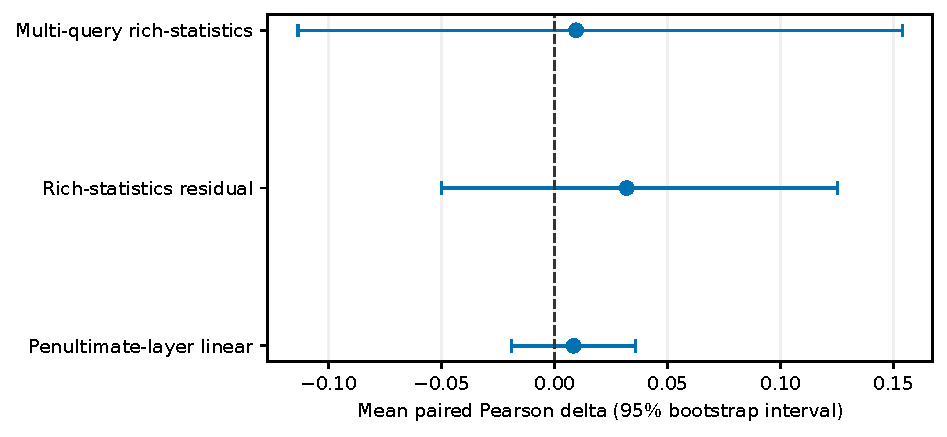
\includegraphics[width=0.82\linewidth]{generated/bootstrap_intervals.pdf}
  \caption{Mean primary Pearson differences and joint 95\% confidence intervals.
  Every interval includes the no-difference line.}
  \label{fig:bootstrap}
\end{figure}

The penultimate-layer and rich-statistics heads improved on every seed. The
multi-query head improved on eight seeds and lost on \MultiQueryLosses{}.
Figure~\ref{fig:seed-deltas} shows these differences. The consistent signs in
the first two comparisons describe training variability on this cohort;
they do not remove uncertainty across participants.

\begin{figure}[tbp]
  \centering
  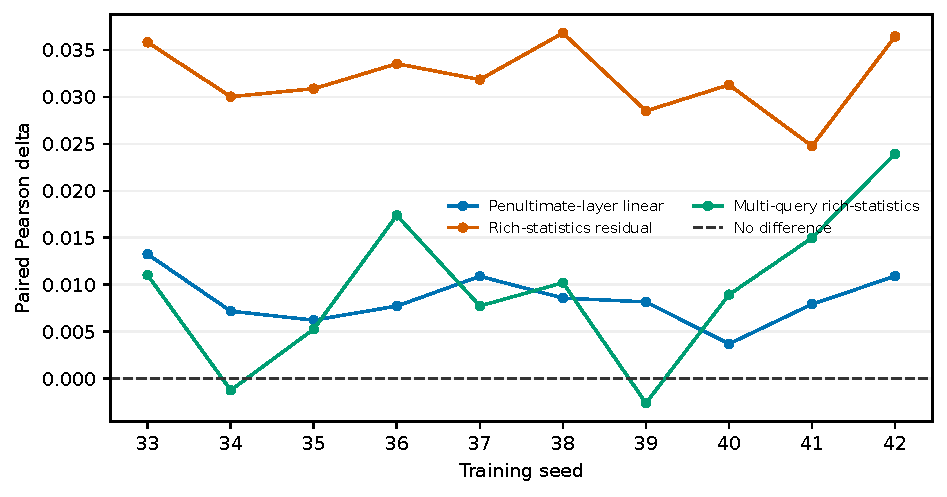
\includegraphics[width=0.86\linewidth]{generated/seed_deltas.pdf}
  \caption{Primary paired Pearson differences by training seed, all evaluated
  on the same 75 participants. Positive values favor the candidate.}
  \label{fig:seed-deltas}
\end{figure}

\subsection{Exploratory training-size analysis}
The 90 runs at 200, 400, and 800 HBN training subjects produced 6,750 predictions
for the same 75 MIPDB participants. Both the rich-statistics and matched MLP
heads had positive mean advantages at every size, with all ten seed differences
positive in each comparison (Figure~\ref{fig:capacity-main}). Their mean
advantages decreased across the tested sizes. The 200-subject intervals were
above zero, while the 800-subject intervals included zero.

Comparing those interval decisions alone does not test whether the effects
changed. Direct 800-minus-200 contrasts were $-0.046$ for the rich head
(95\% CI $[-0.112,0.023]$) and $-0.039$ for the MLP
($[-0.090,0.012]$). Both included zero. One adjacent MLP contrast, 800 minus
400, had an interval below zero ($[-0.061,-0.004]$); its one-sided test of a
positive change gave an adjusted p-value of 1.000. These exploratory results
are reported in full in Appendix~\ref{sec:capacity}; they do not establish a
universal scaling law.

\begin{figure}[tbp]
  \centering
  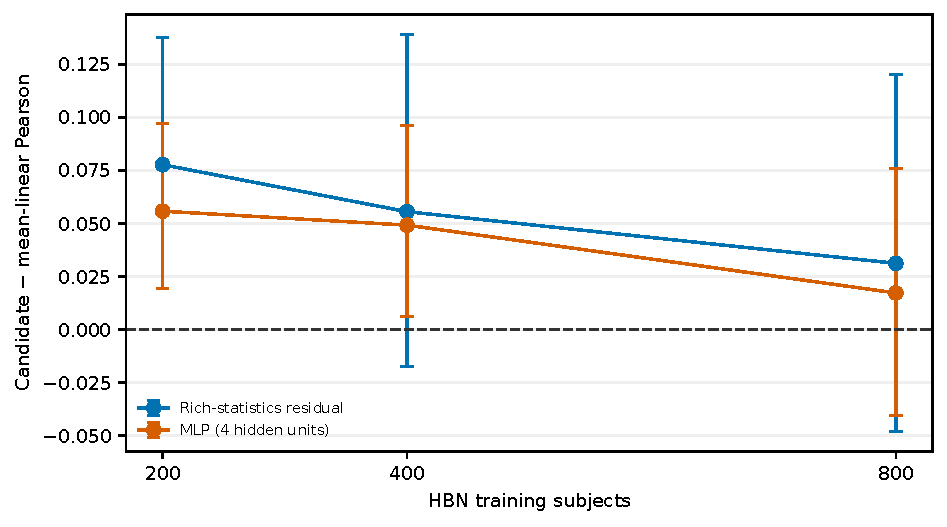
\includegraphics[width=0.86\linewidth]{presentation/capacity_data_regime_delta.pdf}
  \caption{Exploratory training-size analysis. Mean paired Pearson differences
  from the size-matched linear baseline, with joint 95\% intervals.}
  \label{fig:capacity-main}
\end{figure}

\subsection{Exploratory layer-wise analysis}
Four linear probes were evaluated across ten seeds on the same
\LayerwiseSubjectCount{} MIPDB participants. Relative to the final-layer
mean-linear baseline, the mean differences were \LayerwiseMFourDelta{},
\LayerwiseMThreeDelta{}, and \LayerwiseMTwoDelta{} at layers $-4$, $-3$, and
$-2$, respectively. All intervals crossed zero (Table~\ref{tab:layerwise}).
The positive estimates do not establish a stable layer advantage or a primary
superiority claim. Figures~\ref{fig:layerwise-depth} and
\ref{fig:layerwise-seed-deltas} in the appendix show the depth and seed patterns.

\begin{table}[tbp]
  \centering
  \small
  \caption{Exploratory layer-wise differences from the final-layer baseline.
  Intervals resample seeds and participants; Holm-adjusted p-values refer to
  seed sign-flip tests.}
  \label{tab:layerwise}
  \begin{tabular}{lrrrrr}
\toprule
Layer & Mean $\Delta r$ & 95\% interval & Holm $p$ & W/T/L & Worst $\Delta r$ \\
\midrule
Layer -4 & 0.042 & [-0.046, 0.151] & 0.003 & 10/0/0 & 0.031 \\
Layer -3 & 0.030 & [-0.015, 0.084] & 0.003 & 10/0/0 & 0.024 \\
Layer -2 & 0.008 & [-0.019, 0.036] & 0.003 & 10/0/0 & 0.004 \\
\bottomrule
\end{tabular}

\end{table}

\subsection{Secondary transfer to ds006780}
The secondary transfer evaluated \DsRunCount{} selected runs on
\DsSubjectCount{} participants, producing \DsPredictionCount{} predictions.
At 200 HBN training subjects, the rich-statistics head had a mean Pearson
difference of \DsSecondaryDelta{} from the baseline, with 95\% interval
[\DsSecondaryCILow{},\,\DsSecondaryCIHigh{}]. At 800 training subjects, the
difference was \DsPrimaryDelta{} and all \DsPrimaryWins{} seed differences
were positive, but its interval also included zero:
[\DsPrimaryCILow{},\,\DsPrimaryCIHigh{}].

The 800-subject interval width was \DsPrimaryCIWidth{}, exceeding the planned
maximum of \DsPrecisionMaxWidth{}. Thus the precision gate failed. The interval
both leaves the direction of the population advantage uncertain and is wider
than intended; this analysis does not establish stable superiority.
Table~\ref{tab:ds006780-summary} and Figure~\ref{fig:ds006780} report the results.

\begin{table}[tbp]
  \centering
  \small
  \caption{Secondary ds006780 transfer. Pearson and seed SD summarize ten
  training runs. Paired differences and joint intervals compare the rich head
  with the baseline at the same training size.}
  \label{tab:ds006780-summary}
  \begin{tabular}{llrrrr}
\toprule
Training $n$ & Head & Pearson & Seed SD & $\Delta r$ & 95\% interval \\
\midrule
200 & Mean-pooled linear & 0.2650 & 0.0141 & -- & -- \\
200 & Rich-statistics residual & 0.2577 & 0.0168 & -0.0073 & [-0.0861, 0.0721] \\
800 & Mean-pooled linear & 0.3255 & 0.0091 & -- & -- \\
800 & Rich-statistics residual & 0.3543 & 0.0107 & 0.0287 & [-0.0349, 0.0922] \\
\midrule
\multicolumn{6}{l}{Precision gate: failed; observed width 0.1272, threshold 0.0600.} \\
\bottomrule
\end{tabular}

\end{table}

\begin{figure}[tbp]
  \centering
  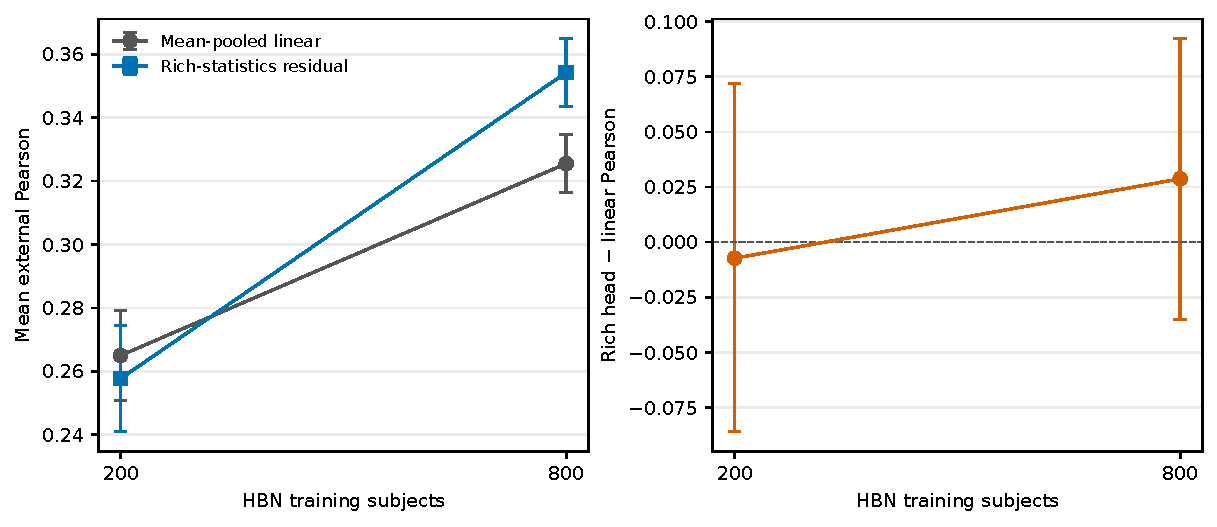
\includegraphics[width=0.95\linewidth]{../results/extensions/ds006780_external_v5/ds006780_external.pdf}
  \caption{Secondary ds006780 results. Left: Pearson correlations with standard
  deviations across seeds. Right: paired differences with intervals that also
  resample participants. Both intervals include zero.}
  \label{fig:ds006780}
\end{figure}

